\section*{Mini-Project 3: AC Wiring in Residential Buildings}
\label{lab_building_wiring}

\fancypagestyle{interlude}[fancy]{%
	\fancyhead[LO,RE]{}
	\fancyhead[LE,RO]{\slshape \MakeUppercase{Mini-Project 3: AC wiring in Residential Buildings}}
}
\addcontentsline{toc}{section}{\hspace{0.35in} \textbullet~Mini-Project 3: AC Wiring in Residential Buildings}
\pagestyle{interlude}

%\makelabheader %(Space for student name, etc., defined in master.tex)

\bigskip

\textbf{Background}

So far, every circuit you have built has used small voltages and currents.  And because you've been focused how the circuits worked, you haven't paid much attention how their pieces were actually held together.  By contrast, this Mini-Project will have you wiring 120-volt circuits capable of carrying up to 15 amps, using the same electrical devices and wiring techniques that you would use if you were rewiring a home.  Our focus will be on safety, reliability, and code-compliance as specified in the US National Electric Code (NEC).

\bigskip
\textbf{Your Task}

As a class, we will construct the circuit pictured on the following page, with each student responsible for building a specific part of the circuit, either individually or working as a pair.  Your instructor will play the role of the county electrical inspector, who must approve of all wiring \textit{before} the device and wiring are folded together and enclosed in the electrical box.  When all parts of the circuit are complete, we will turn it on and verify that it works as intended---including an actual test that the GFCI is functional.

For this lab, you do not need to write anything in your lab note notebook, and you will not be asked to turn anything in.  Your only jobs are to learn and have fun.


\bigskip
\textbf{Details for New Work Boxes}

Any electrical boxes that are already screwed to the wooden frames (made of \textit{studs}) at your station are \textit{new work} boxes.  Here, you are to imagine that you are constructing a new building or new room, and that you are installing the electrical work before any drywall is put up.  Here are the steps to do, in this specific order:
\begin{enumerate}
\item Remove the smallest number of knockout tabs needed for cables to enter the box. (They might have been removed already.)  
\item Insert cables into the back of the box.
\item Make all connections between wires and any devices that will go inside the box, but leave everything hanging outside of the box for now.
\item Secure all cables to studs with staples.
\item Have all of your wiring inspected by your instructor.
\item \textit{After} you have passed inspection, screw a piece of (fake) drywall to the stud around the electrical box.
\item Fold all wires into the box, screw your device into the box, and install a white cover plate over it if needed.
\end{enumerate}

\medskip \textbf{Details for Old Work Boxes}

Any place at your station where an 8-inch square of drywall (actually plywood) is already attached to a stud is meant for an  \textit{old work} box.   Here, you are imagining that the drywall is already in place and that you are merely \textit{adding} a new outlet, switch, or light fixture to the room.  Here are the steps to do, in this specific order:

\begin{enumerate}
\item Do not remove any clamps from back of new work boxes.  They are not knockouts!
\item Insert cables through the back of the rectangular opening in the fake drywall.
\item Insert cables through back of electrical box and mount box into the opening that is cut in the fake drywall.
\item Make all connections between wires and any devices that will go inside the box, but leave everything hanging outside  of the box for now.  
\item Have all wiring inspected by your instructor.
\item Fold wires into box, screw device into box, and install the white cover plate over it if needed.
\end{enumerate}
\newpage

\begin{center}
\raisebox{0pt}{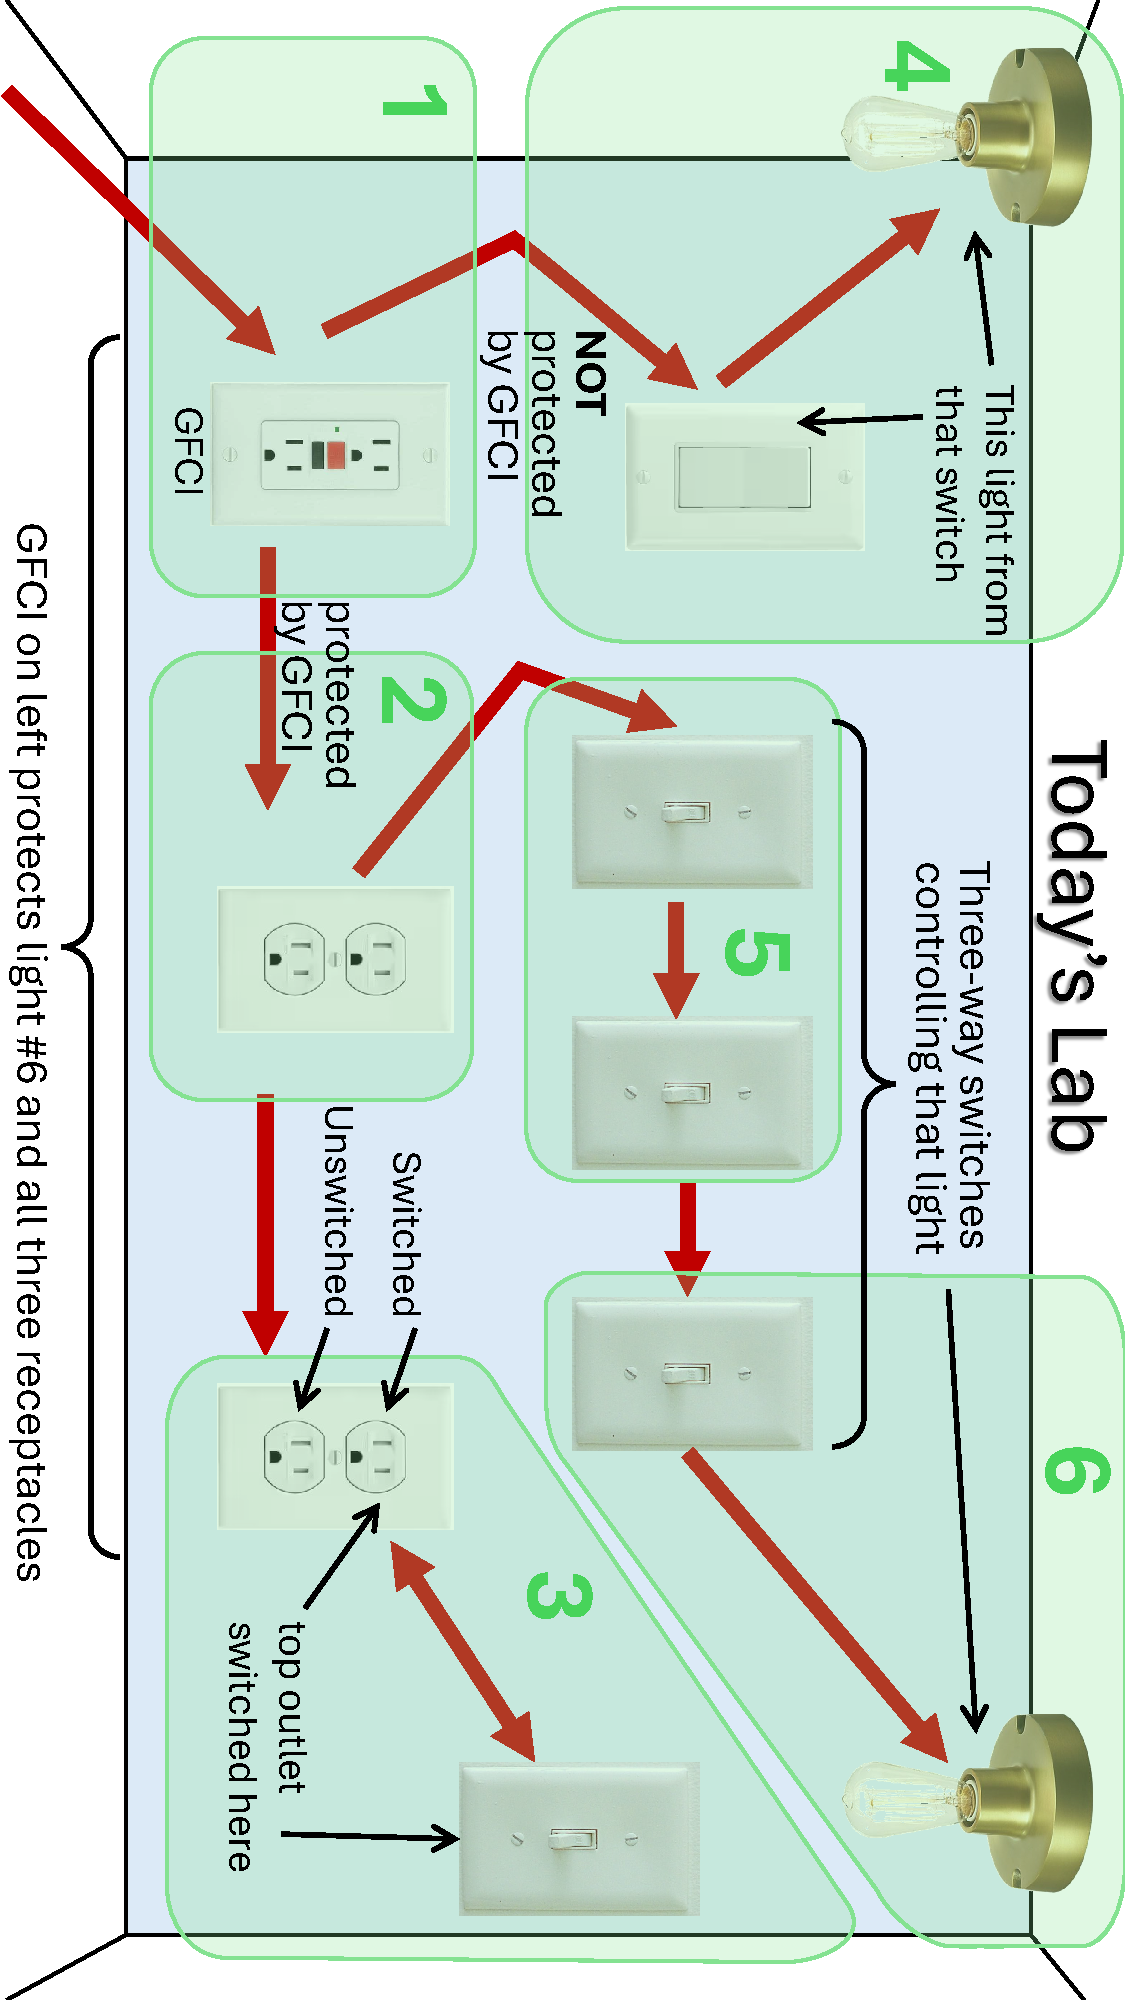
\includegraphics[scale=0.67]{building_wiring/building_wiring_lab.pdf}}
\end{center}

